
\documentclass[conference]{IEEEtran}
\IEEEoverridecommandlockouts
% The preceding line is only needed to identify funding in the first footnote. If that is unneeded, please comment it out.
\usepackage{cite}
\usepackage{amsmath,amssymb,amsfonts}
\usepackage{algorithmic}
\usepackage{graphicx}
\usepackage{textcomp}
\usepackage{xcolor}
\usepackage{multirow}
\usepackage{amssymb,amsthm}
\usepackage{amsmath}
\usepackage{float}
\usepackage{glossaries}
\usepackage{subcaption}  % Untuk subfigure
\usepackage{pdfpages}
\def\BibTeX{{\rm B\kern-.05em{\sc i\kern-.025em b}\kern-.08em
    T\kern-.1667em\lower.7ex\hbox{E}\kern-.125emX}}

\usepackage{listings}

\begin{document}

\title{Continuous and Adjustable Interaction Style of Explanatory Robot}

\author{\IEEEauthorblockN{Alvin N. Atmadja}
\IEEEauthorblockA{\textit{Department of Electrical Engineering} \\
\textit{National Taiwan Normal University}\\
Taipei, Taiwan \\
61575083H@ntnu.edu.tw}
\and
\IEEEauthorblockN{Matthew Exon}
\IEEEauthorblockA{\textit{Department of Electrical Engineering} \\
\textit{National Taiwan Normal University}\\
Taipei, Taiwan \\
61575084H@ntnu.edu.tw}
\and
\IEEEauthorblockN{ Elham Feilizadeh}
\IEEEauthorblockA{\textit{Department of Electrical Engineering} \\
\textit{National Taiwan Normal University}\\
Taipei, Taiwan \\
elhamfeilizadeh@gmail.com}
\and
\IEEEauthorblockN{ Salar Mokhtari Laleh}
\IEEEauthorblockA{\textit{Department of Electrical Engineering} \\
\textit{National Taiwan Normal University}\\
Taipei, Taiwan \\
61375091h@ntnu.edu.tw}
}

\maketitle

% \begin{abstract}

% \end{abstract}

% \begin{IEEEkeywords}
% \textit{State-Space}, \textit{Cruise Control}, LQR, \textit{Pole-Placement}, Linearisasi
% \end{IEEEkeywords}

\section{Introduction}

Recent research has led to the development of an autonomous museum robot designed to facilitate interactive and personalised guided tours for museum visitors. The developed system is capable of autonomously performing several key functions required for effective human–robot interaction in museum environments. Specifically, the robot can:

\begin{enumerate}
    \item Provide guided tours to individual visitors.
    \item Detect and recognise a visitor’s consent and willingness to participate in a guided tour.
    \item Autonomously navigate the museum and lead visitors to exhibits in an appropriate sequence.
    \item Understand and respond to visitor queries related to the exhibits.
    \item Deliver verbal descriptions and relevant information about the exhibits currently being presented.
\end{enumerate}
This platform provides a strong foundation for further investigation into autonomous museum guide robots and human–robot interaction. Building upon the existing system, research can evaluate the robot’s performance through real-world interactions with museum visitors, with particular emphasis on user experience, perceived usefulness, naturalness of interaction, engagement, and overall satisfaction.

During guided tours, visitors’ feedback and behavioural responses can be systematically collected and analysed to identify limitations in the current system and determine opportunities for improvement. These findings can subsequently inform the design and development of more effective, adaptive, and visitor-centred robotic guidance systems. Such an iterative approach can contribute to the advancement of socially intelligent museum robots capable of delivering more engaging, responsive, and personalised experiences for diverse visitors.


\subsection{Purpose of the research}

We want to answer the following research question:
\begin{itemize}
    \item How can small talk help a robot adjust its manner and enhance the visit enjoyment of a museum visitor?
\end{itemize}

\subsection{Scope of Problems and Assumptions}

The assumption of our project is as stated below:
\begin{enumerate}
    \item The hallway is assumed to be straight.
    \item The robot is assumed to have approximately 1 m/s speed.
    \item An LLM has sufficient capability to interpret the mood of the guest from small talk and adjust the talking style based accordingly
    \item The robot need only talk to one person at a time.
    \item Visitors can broadly be characterised by three personas, included in this paper in the Appendix \ref{Appendix-Persona}.
\end{enumerate}

The scope of the problem of our project is as stated below:
\begin{enumerate}
    \item The robot will only accompany guests that consent to using a robot guide.
    \item Guests that consent will be classified into two groups: those that like robots and those that do not. This can be detected by the response of the guest during the small talk session.
    \item While engaged in small talk, the robot does not need to try to see the guest's eyes.
    \item Movements of the robot are not reviewed.
    \item Changing the talking style of the robot (the sentence structure, or the words come out of the robot) is the main focus.
    \item The voice of the robot and the expression on the robot's voice are not reviewed.
    \item While explaining the exhibits, the robot will not engage in small talk, but rather focus on explaining.
\end{enumerate}

\subsection{Constructs}

Our research construct relies on these theories. 

\begin{enumerate}
\item Small Talk\cite{ren1}
: A conversational style involving the exchange of short questions and
  answers concerning topics of relatively low emotional or cognitive
  load.
\item Robot Acceptance\cite{syrdal1}
: The degree to which a human interacting with a robot accepts the
  presence of the robot as a natural part of their environment, rather
  than a source of stress or discomfort.
\item Affect\cite{picard1}
: The underlying emotional state of a person, as it influences their manner of communication.
\item Visit Enjoyment\cite{othman1}
: The extent to which a visitor to a museum derives both short term
  enjoyment while visiting, as well as the subsequent benefit the
  visitor receives from having visited the museum in the past.
\end{enumerate}

\section{Testing Method}

We test our robot in a certain virtual environment/scenario, which explained as below:

\begin{enumerate}
    \item We will test our robot in a straight hallway in which hang several exhibits, either paintings or other artifacts.
    \item The distance of each exhibit to another is random, but some distances exceed a certain threshold, allowing the robot to engage small talk between exhibits. 
    \item Variable t 
    \item Every exhibit will be named with variable $p_1$, $p_2$, and so on.
    \item The first point of the robot is $p_0$, which is the point where the robot welcomes the guest. 
\end{enumerate}

The robot process is described as in the flowchart in Figure \ref{fig:tstingMethod-flowchartRobot}.

\clearpage
\begin{figure*}[p]
    \centering
    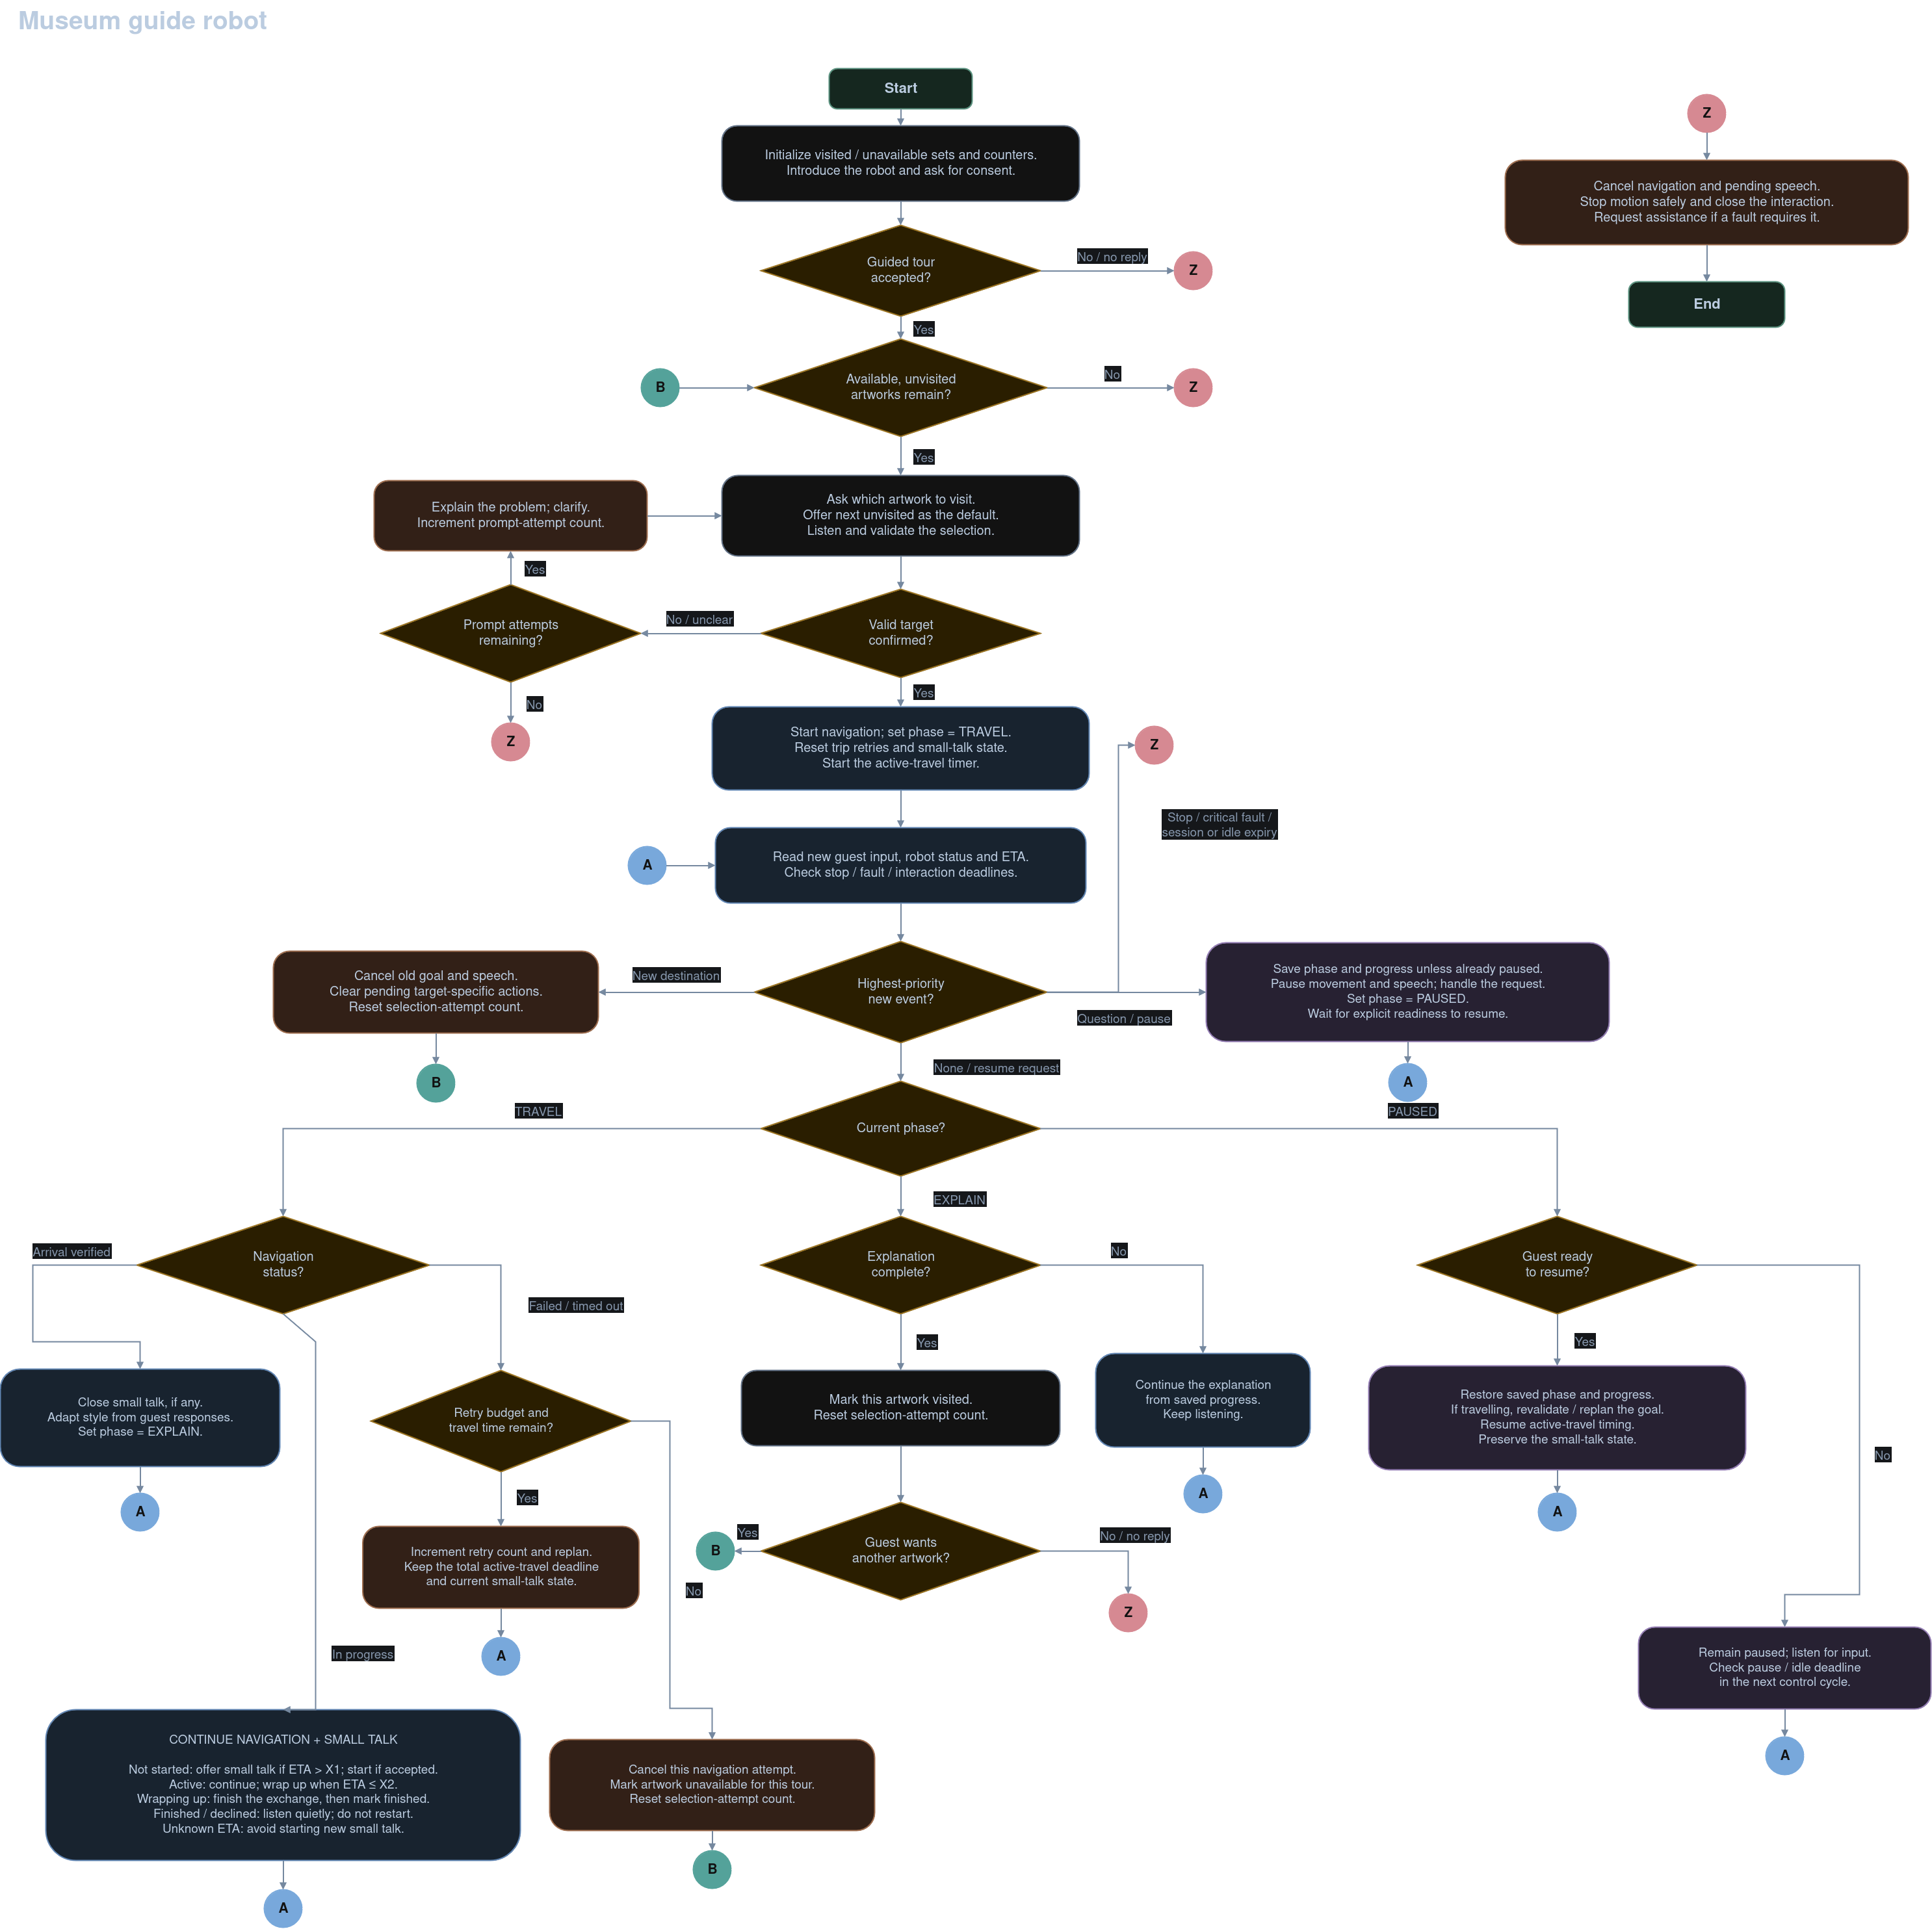
\includegraphics[
        width=\textwidth,
        height=0.90\textheight,
        keepaspectratio
    ]{Pictures/Fig1.png}
    \caption{Flowchart of Small Talk in the Robot}
    \label{fig:tstingMethod-flowchartRobot}
\end{figure*}
\clearpage

\section{Method of Survey}

We will use previously established survey questions to evaluate the museum visitor's experience.

\begin{enumerate}
    \item Negative Attitude towards Robots Scale (NARS)\cite{syrdal1}
    \item Museum Experience Scale\cite{othman1}
\end{enumerate}

NARS will be used to evaluate the visitor's attitude towards robots generally.  This should act as a benchmark to retrospectively evaluate the robot's real-time evaluation of the visitor's reaction.

MES will be used to evaluate the overall outcome of the visitor's tour.  The overall intent of this research is to improve the quality of the visitor's experience, which will be measured by this scale.  We will adapt this scale by only including the first two sections, omitting sections more concerned specifically with multimedia exhibits.

We will combine these two measures in order to determine the effect on the overall outcome of:

\begin{enumerate}
    \item The visitor's attitude to robots
    \item The robot correctly identifying the visitor's attitude, and adjusting its responses
    \item The robot misidentifying the visitor's attitude.
\end{enumerate}

\section{Literature Review}

\bibliographystyle{ieeetr} % Specify the bibliography style
\bibliography{2referencesbib} % Reference the .bib file

\newpage
\appendices
\newpage
\section{Persona}
\label{Appendix-Persona}
There are three personas used in this research. 
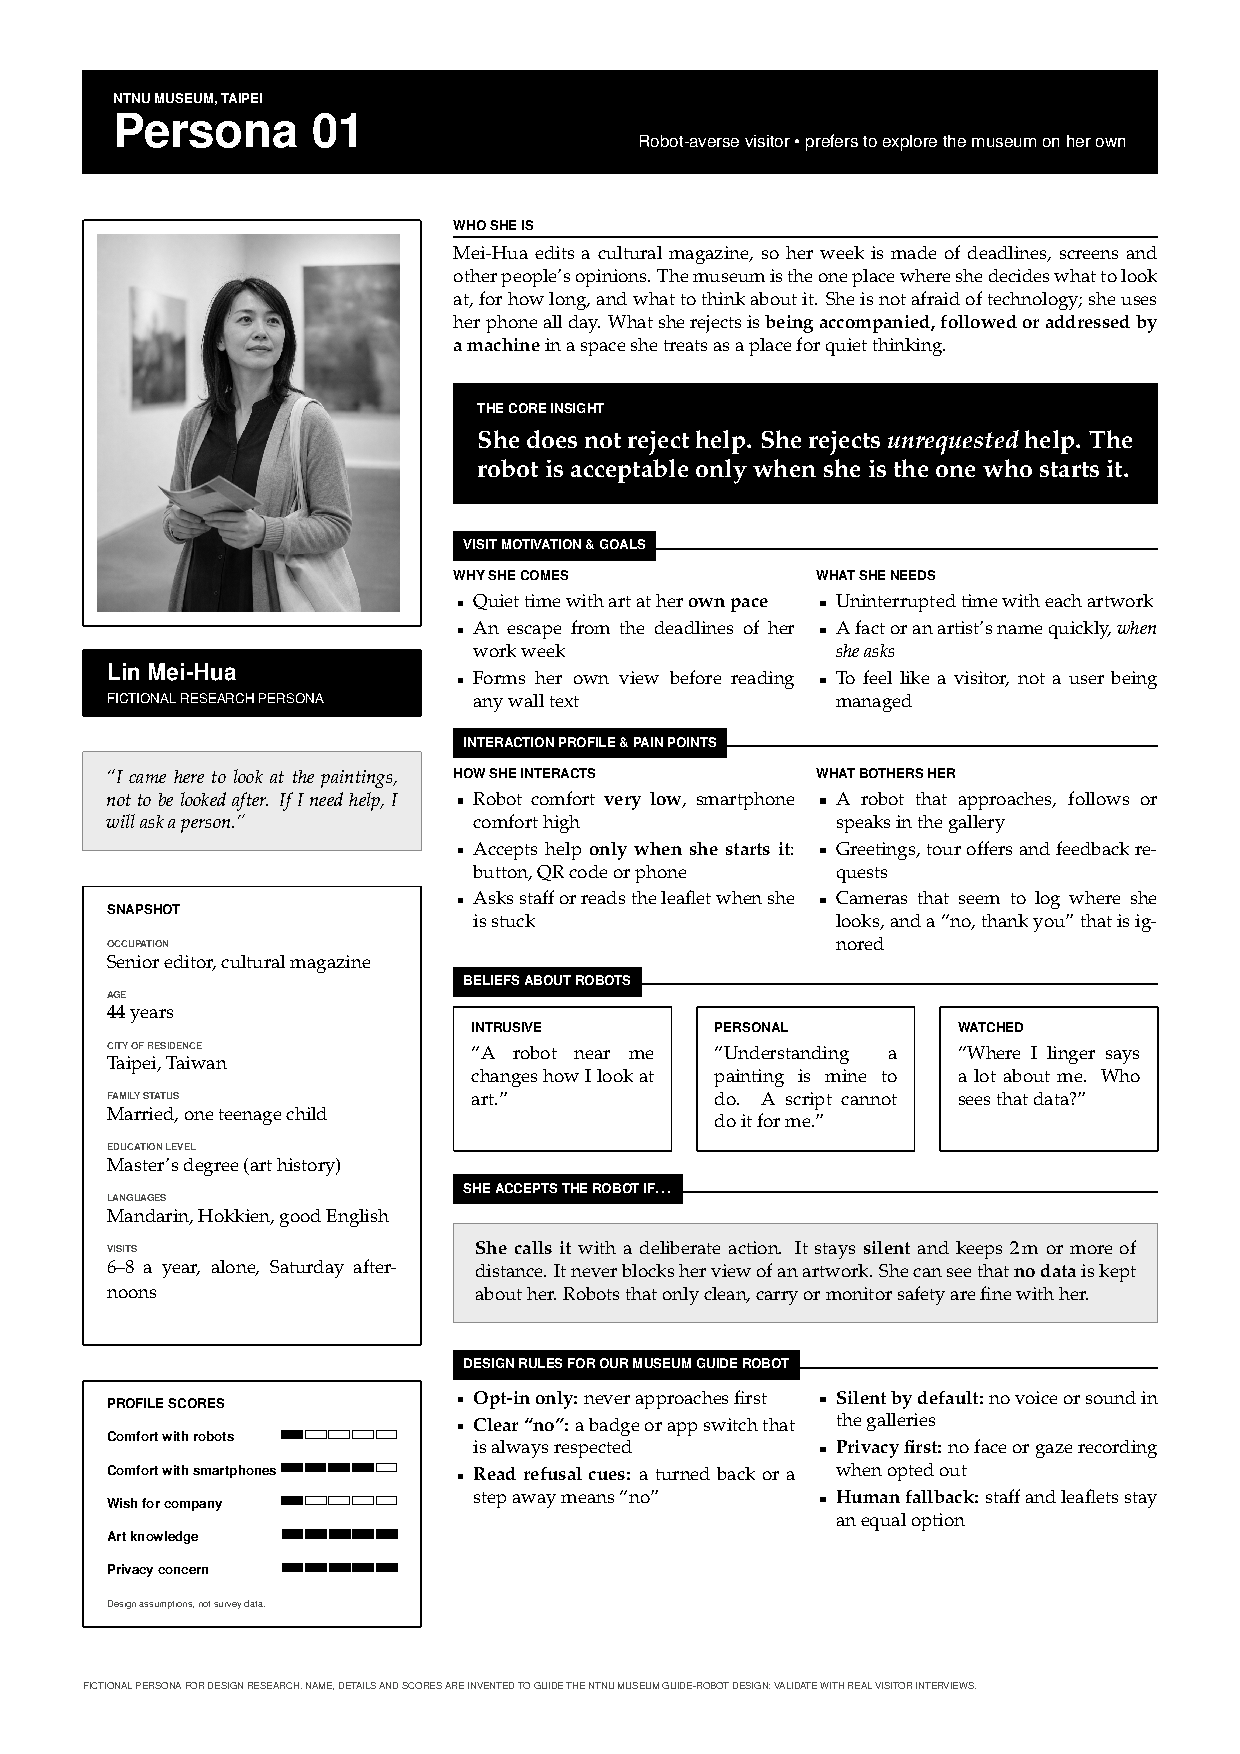
\includepdf[pages=-]{pdfs/persona01.pdf}
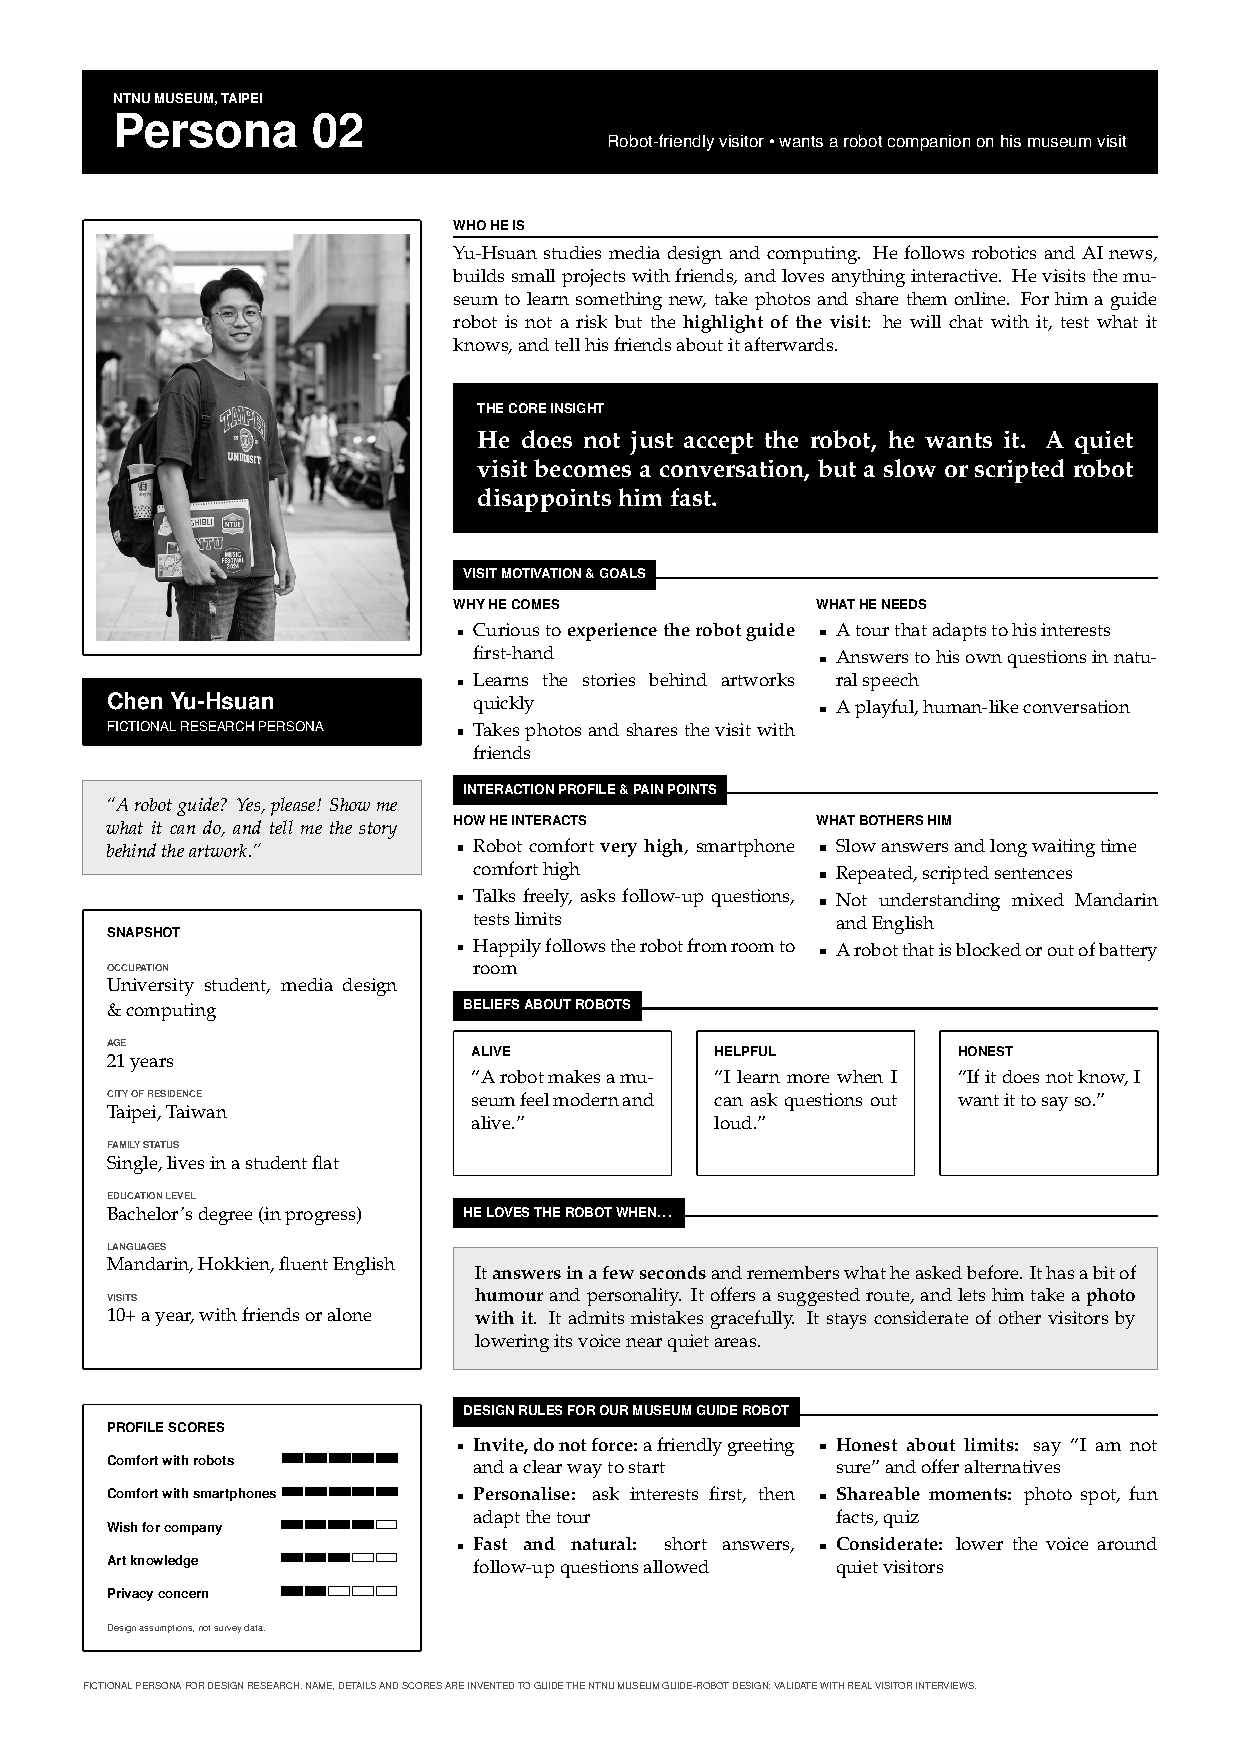
\includepdf[pages=-]{pdfs/persona02.pdf}
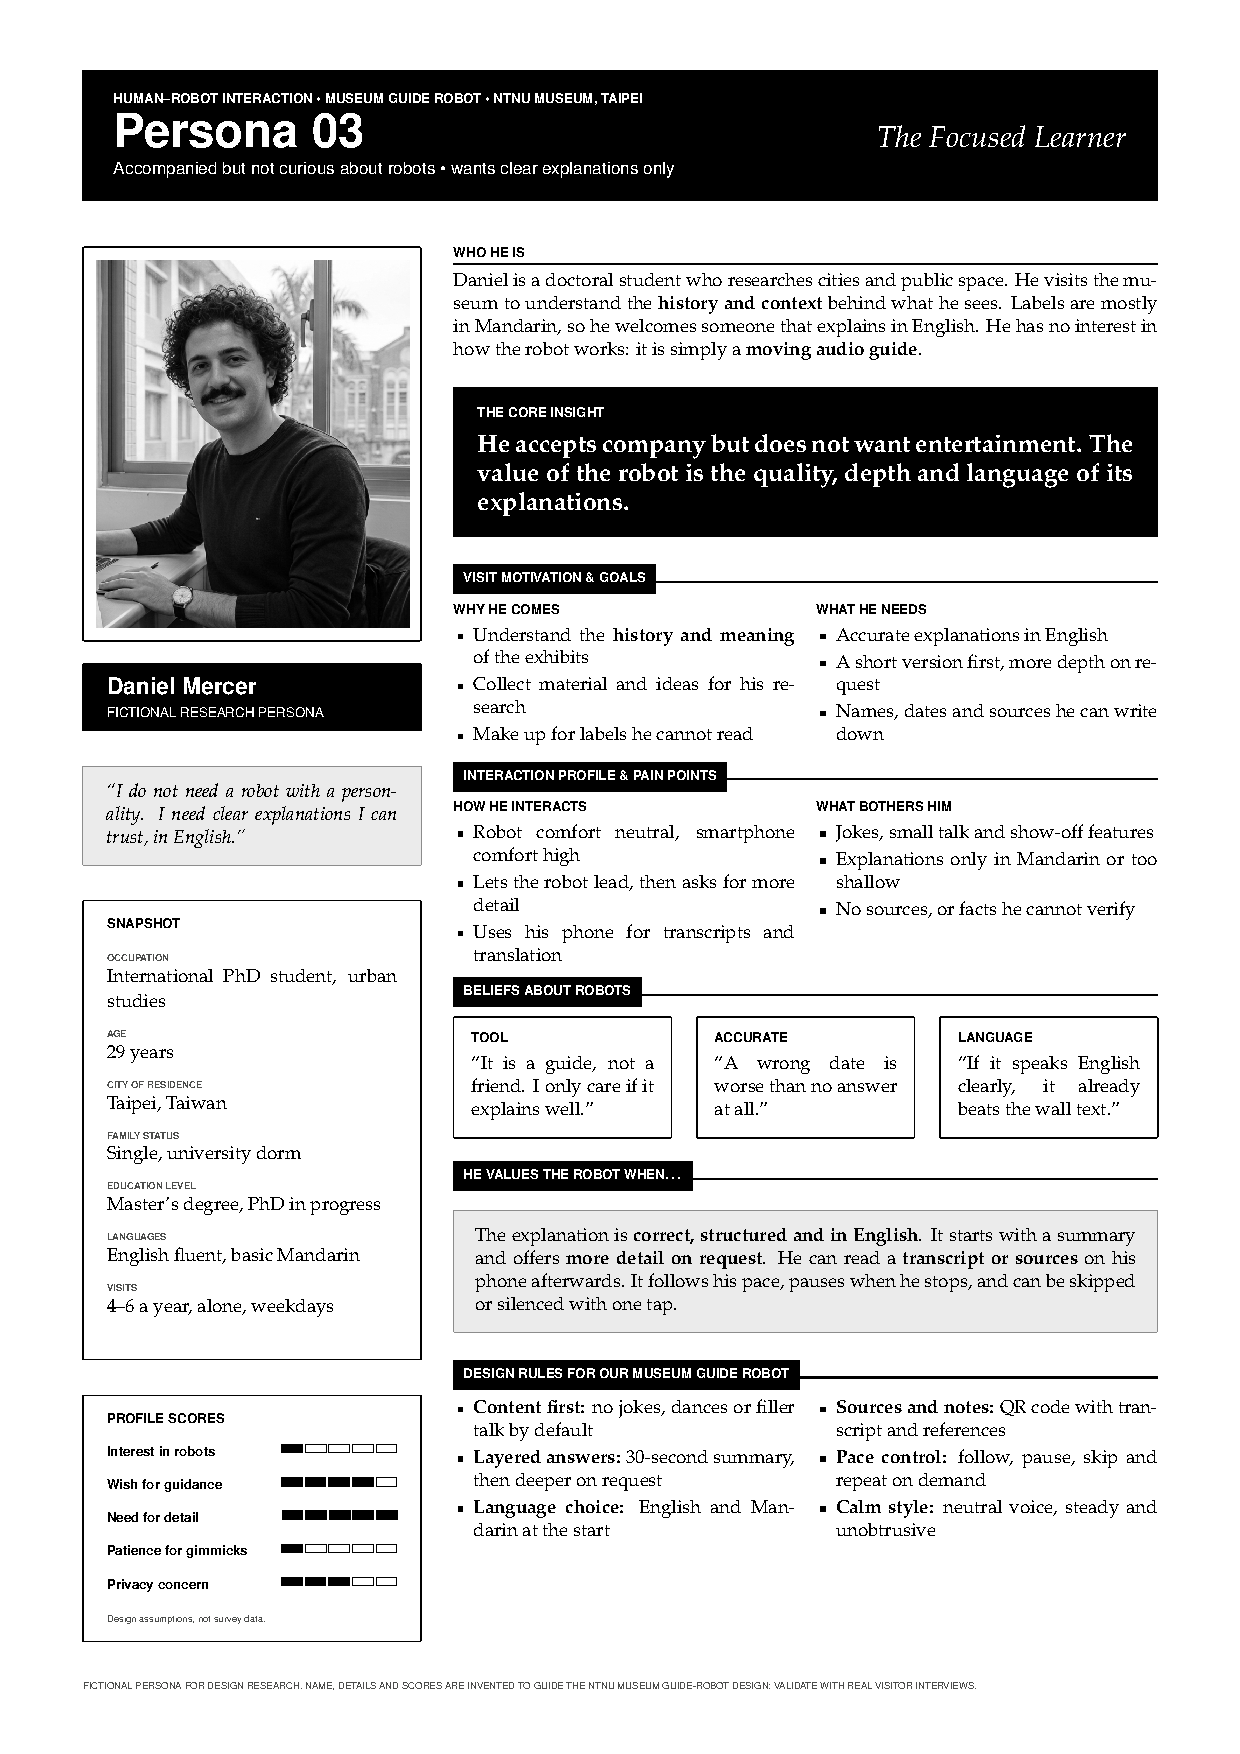
\includepdf[pages=-]{pdfs/persona03.pdf}

\end{document}






































































% \begin{enumerate}
%     \item Sistem tidak mempunyai \textit{delay} sama sekali dan tidak ada \textit{first order lag}.
%     \item Gaya selain gaya gesek, gaya beban mobil, dan gaya akibat angin, tidak ditinjau.
%     \item Hal-hal yang terjadi pada mesin dari mobil tidak ditinjau, seperti pedal gas dan rem. 
% \end{enumerate}


% Dalam pembuatan sistem \textit{cruise control}, dilakukan peninjauan pustaka mengenai sistem \textit{cruise control}. Kebanyakan model sistem \textit{cruise control} yang ditinjau menggunakan contoh mobil. Dalam hal ini mobil yang ditinjau berada di sebuah tanjakan yang konstan sudutnya dengan gaya yang dikenakan ke mobil adalah gaya hambatan angin \eqref{eq:bab1-fd}, gaya gesek \eqref{eq:bab1-ff}, dan gaya beban mobil \eqref{eq:bab1-fg}. Gambar \ref{fig:bab1-dbbsistem} adalah Diagram Benda Bebas (DBB) sistem yang ditinjau \cite{utama1,utama2-osman,utama2-prakash,utama2-rout,utama2-vedam}. 

% \begin{figure}[htbp]
%     \centering
%     \includegraphics[width=0.35\textwidth]{S_Gambar/sistem.png}
%     \caption{Diagram Benda Bebas Sistem yang Ditinjau}
%     \label{fig:bab1-dbbsistem}
% \end{figure}

% \begin{eqnarray}
%     F_d &=& c_d(v_{angin}+v_{mobil})^2 \label{eq:bab1-fd}\\
%     F_f &=& c_f  m  g  cos(\theta)\label{eq:bab1-ff}\\
%     F_f &=& m g sin(\theta)\label{eq:bab1-fg}
% \end{eqnarray}

% \noindent Keterangan:
% \begin{align*}
%     &\theta &= & \text{Sudut tanjakan}\\
%     &c_f &= & \text{Konstanta gesek}\\
%     &c_d &= & \text{Konstanta \textit{drag} (${Kg}/{m}$)}\\
%     &m &= & \text{Massa Benda (\textit{Kg})}\\
%     &g &= & \text{Gravitasi (${m}/{s^2}$)}\\
%     &v_{angin} &= & \text{Kecepatan angin (${m}/{s}$)}\\
%     &v_{mobil} &= & \dot{x}(t) = \text{Kecepatan mobil (${m}/{s}$)}\\
%     &f(t) &= & \text{Gaya Mobil (\textit{N})}
% \end{align*}


% Model keadaan ruang/\textit{state-space} adalah model matematika yang merepresentasikan sistem fisik dan mendeksripsikan perilaku sistem dalam variabel keadaan atau \textit{state-variable}. Persamaan umum dari model keadaan ruang adalah persamaan keadaan atau \textit{state-equation} \eqref{eq:bab1-stateeq} dan persamaan output atau \textit{output-equation} \eqref{eq:bab1-outeq}\cite{buku-ogata2010modern,buku2-wade2004basic,cc-app3}. 

% \begin{eqnarray}
%    \mathbf{\dot{x}} &=& \mathbf{Ax+Bu} \label{eq:bab1-stateeq}\\
%     \mathbf{y} &=& \mathbf{Cx}\label{eq:bab1-outeq}
% \end{eqnarray}

% \noindent Keterangan:
% \begin{align*}
%     &n &= & \text{Orde tertinggi persamaan differensial}\\
%     &\mathbf{A} &= & \text{Matriks nxn}\\
%     &\mathbf{B} &= & \text{Matriks nxm}\\
%     &\mathbf{C} &= & \text{Matriks nxn}\\
%     &\mathbf{u} &= & \text{Vektor input}\\
%     &\mathbf{x} &= & \text{Vektor keadaan}\\
%     &\mathbf{y} &= & \text{Vektor output}
% \end{align*}

% \eqref{eq:bab1-linearisasi}.

% \begin{equation}
%     \begin{split}
%         \text{A} &= \frac{\delta f(x(t),u(t))}{\delta x(t)} \bigg|_{x^*(t),u^*(t)}\\
%         \text{B} &= \frac{\delta f(x(t),u(t))}{\delta u(t)} \bigg|_{x^*(t),u^*(t)}\\
%         \text{C} &= \frac{\delta g(x(t),u(t))}{\delta x(t)} \bigg|_{x^*(t),u^*(t)}\label{eq:bab1-linearisasi}
%     \end{split}
% \end{equation}




% \begin{equation}
%     \mathbb{C} = 
%     \begin{bmatrix}
%     \mathbf{B} & \mathbf{AB} &\mathbf{ A^2B} & ... & \mathbf{A^{\textit{n}-1}B}  \label{eq:bab1-controlability}
%     \end{bmatrix}
% \end{equation}


% \begin{equation}
%     \mathbb{O} = 
%     \begin{bmatrix}
%     \mathbf{C} \\ \mathbf{CA} \\ \mathbf{CA^2} \\ ... \\ \mathbf{CA^{\textit{n}-1}}  \label{eq:bab1-observability}
%     \end{bmatrix}
% \end{equation}








% \begin{equation}
% \resizebox{0.4\textwidth}{!}{%
%     \begin{split}
%             \begin{bmatrix}
%     \dot{x_1}\\\dot{x_2}
%     \end{bmatrix}
%     &=&
%     \begin{bmatrix}
%     0 & 1\\0 & -0,0132
%     \end{bmatrix}    
%     \begin{bmatrix}
%     {x_1}\\{x_2}
%     \end{bmatrix}&
%     +
%     \begin{bmatrix}
%     0\\ -9,7358
%     \end{bmatrix}
%     u(t)\\
%     y &=&
%     \begin{bmatrix}
%     0 & 1
%     \end{bmatrix}
%     \begin{bmatrix}
%     {x_1}\\{x_2}
%     \end{bmatrix}&  \label{eq:bab2-stateeq-linearize-withconstanta}  
%     \end{split}}
% \end{equation}

% \begin{align*}
% R &=10^{-8}\\
%     \mathbf{Q} &= \begin{bmatrix}
%         1 &0\\0&{10^{-5}}
%     \end{bmatrix}
% \end{align*}
    
% \begin{align*}
% R &=10\\
%     \mathbf{Q} &= \begin{bmatrix}
%         1 &0\\0&{10^{-5}}
%     \end{bmatrix}
% \end{align*}

% \begin{align*}
% R &=10^{-8}\\
%     \mathbf{Q} &= \begin{bmatrix}
%         1 &0\\0&{2}
%     \end{bmatrix}
% \end{align*}





% %-====================
% \section{Kode MATLAB untuk Pengujian}
% \label{lamp:pengujian}

% \begin{lstlisting}[language=C++, caption={Kode Pengujian Kestabilan, Keterkontrolan, dan Keteramatan}]

% \end{lstlisting}

% %-====================
% \section{Kode MATLAB untuk Pengontrol Sistem dengan Metode LQR}
% \label{lamp:lqr}


% \begin{lstlisting}[language=C++, caption={Pengontrol Sistem dengan Metode LQR}]

% \end{lstlisting}

% %-====================

% \section{Kode MATLAB untuk Pengontrol Sistem dengan Metode \textit{Pole-Placement}}
% \label{lamp:pole}

% \begin{lstlisting}[language=C++, caption={Pengontrol Sistem dengan Metode \textit{Pole-Placement}}]

% \end{lstlisting}


% %-====================
% \section{Tambahan Kode MATLAB untuk Simulasi dengan Sinyal Input Berbeda}
% \label{lamp:kode-tambahan}


% \begin{lstlisting}[language=C++, caption={Tambahan Simulasi Kode MATLAB}]

% \end{lstlisting}
% \end{document}
